\documentclass[10.7pt, twocolumn]{article}

\usepackage[letterpaper, margin=2.54cm, top=2.54cm]{geometry}
\usepackage[super,comma,sort&compress]{natbib}
\usepackage{lmodern}
\usepackage{authblk} % To add affiliations to authors
\usepackage{amssymb,amsmath}
\usepackage{wrapfig}
\usepackage{graphicx,grffile}
\usepackage[labelfont=bf,labelsep=period]{caption}
\usepackage{ifxetex,ifluatex}
\usepackage{fixltx2e} % provides \textsubscript
\ifnum 0\ifxetex 1\fi\ifluatex 1\fi=0 % if pdftex
  \usepackage[T1]{fontenc}
  \usepackage[utf8]{inputenc}
\else % if luatex or xelatex
  \ifxetex
    \usepackage{mathspec}
  \else
    \usepackage{fontspec}
  \fi
  \defaultfontfeatures{Ligatures=TeX,Scale=MatchLowercase}
    \setmainfont[]{Times New Roman}
    \setsansfont[]{Century Gothic}
    \setmonofont[Mapping=tex-ansi]{Consolas}
\fi
% use upquote if available, for straight quotes in verbatim environments
\IfFileExists{upquote.sty}{\usepackage{upquote}}{}
% use microtype if available
\IfFileExists{microtype.sty}{%
	\usepackage{microtype}
	\UseMicrotypeSet[protrusion]{basicmath} % disable protrusion for tt fonts
}{}

\usepackage{float}
\usepackage{lipsum}
\newtheorem{exm}{Example}


%==============================
% Customization to make the output PDF 
% look similar to the MS Word version
%==============================
% To prevent hyphenation
\hyphenpenalty=10000
\exhyphenpenalty=10000

% To set the sections font size
\usepackage{sectsty}
\allsectionsfont{\fontsize{10}{10}\selectfont}
%\sectionfont{\fontsize{10}{10}\selectfont}
\subsectionfont{\itshape\bfseries\fontsize{10}{10}\selectfont}
\subsubsectionfont{\normalfont\itshape}

% No new line after subsubsection
\makeatletter
\renewcommand\subsubsection{\@startsection{subsubsection}{3}{\z@}%
	{-3.25ex\@plus -1ex \@minus -.2ex}%
    {-1.5ex \@plus -.2ex}% Formerly 1.5ex \@plus .2ex
    {\normalfont\itshape}}
\makeatother

\makeatletter % Reference list option change
\renewcommand\@biblabel[1]{#1.} % from [1] to 1
\makeatother %

% To set the doc title font
\usepackage{etoolbox}
\makeatletter
\patchcmd{\@maketitle}{\LARGE}{\bfseries\fontsize{15}{16}\selectfont}{}{}
\makeatother

% No page numbering
\pagenumbering{gobble}

\makeatletter
\def\maxwidth{\ifdim\Gin@nat@width>\linewidth\linewidth\else\Gin@nat@width\fi}
\def\maxheight{\ifdim\Gin@nat@height>\textheight\textheight\else\Gin@nat@height\fi}
\makeatother

% Scale images if necessary, so that they will not overflow the page
% margins by default, and it is still possible to overwrite the defaults
% using explicit options in \includegraphics[width, height, ...]{}
\setkeys{Gin}{width=\maxwidth,height=\maxheight,keepaspectratio}
\setlength{\parindent}{0pt}
\setlength{\parskip}{6pt plus 2pt minus 1pt}
\setlength{\emergencystretch}{3em}  % prevent overfull lines
\providecommand{\tightlist}{%
  \setlength{\itemsep}{0pt}\setlength{\parskip}{0pt}}
\setcounter{secnumdepth}{0}
% Redefines (sub)paragraphs to behave more like sections
\ifx\paragraph\undefined\else
\let\oldparagraph\paragraph
\renewcommand{\paragraph}[1]{\oldparagraph{#1}\mbox{}}
\fi
\ifx\subparagraph\undefined\else
\let\oldsubparagraph\subparagraph
\renewcommand{\subparagraph}[1]{\oldsubparagraph{#1}\mbox{}}
\fi
%==============================
\usepackage{hyperref}
\hypersetup{
	unicode=true,
	pdftitle={NLP4Heatlh_Assignment3_Halim},
	pdfauthor={Jule Valendo Halim - 1425567},
	pdfkeywords={keyword1, keyword2},
	pdfborder={0 0 0},
	breaklinks=true
}
\urlstyle{same}  % don't use monospace font for urls
%==============================

% reduce space between title and begining of page
\title{\vspace{-2em} Investigating the Use of Statistical Tests in Machine Learning Models}
\author[ ]{\bf\fontsize{13}{14}\selectfont Jule Valendo Halim -1425567\vspace{-.7em}}
\affil[ ]{\bf\fontsize{13}{14}\selectfont University of Melbourne}
\date{} % add no date (by default date is added)

%==============================
\begin{document}
\maketitle
\vspace{-4em} %separation between the affiliations and abstract
%==============================

%==============================
\section{Abstract}\label{abstract}
%==============================
\subsection{Objective}

\subsection{Materials}

\subsection{Methods}

\subsection{Results}

\subsection{Discussion}

\subsection{Conclusion}

%==============================
\section{Introduction}\label{introduction}
%==============================
Statistical tests are a popular and long-standing method in multiple fields of science. However, studies in natural language processing (NLP) and machine learning (ML) do not generally include statistcal testing as part of their model evaluation. A survey on 233 published papers in the field of NLP showed that 132 of these papers did not report statistical significance\cite{statsPaper}. However, more studies have begun advocating for the use of these tests to show that experimental results are not coincidental\cite{statsPaper} and argue that a combination of NLP and statistical tests can provide a framework for the development of robust, high-throughput health NLP systems\cite{10.1197/jamia.M3028}. 

In this report, I aim to investigate the use of statistical tests on ML models that predict multi-label and multi-class  classification tasks using the statistical test workflow suggested by Rainio, Tauho, and Klén\cite{statsBased}, as seen in figure \ref{fig:statistical test workflow}. However, instead of comparing results from different test sets, this report compares different model feature inputs.

\begin{figure}[H]
  \centering
  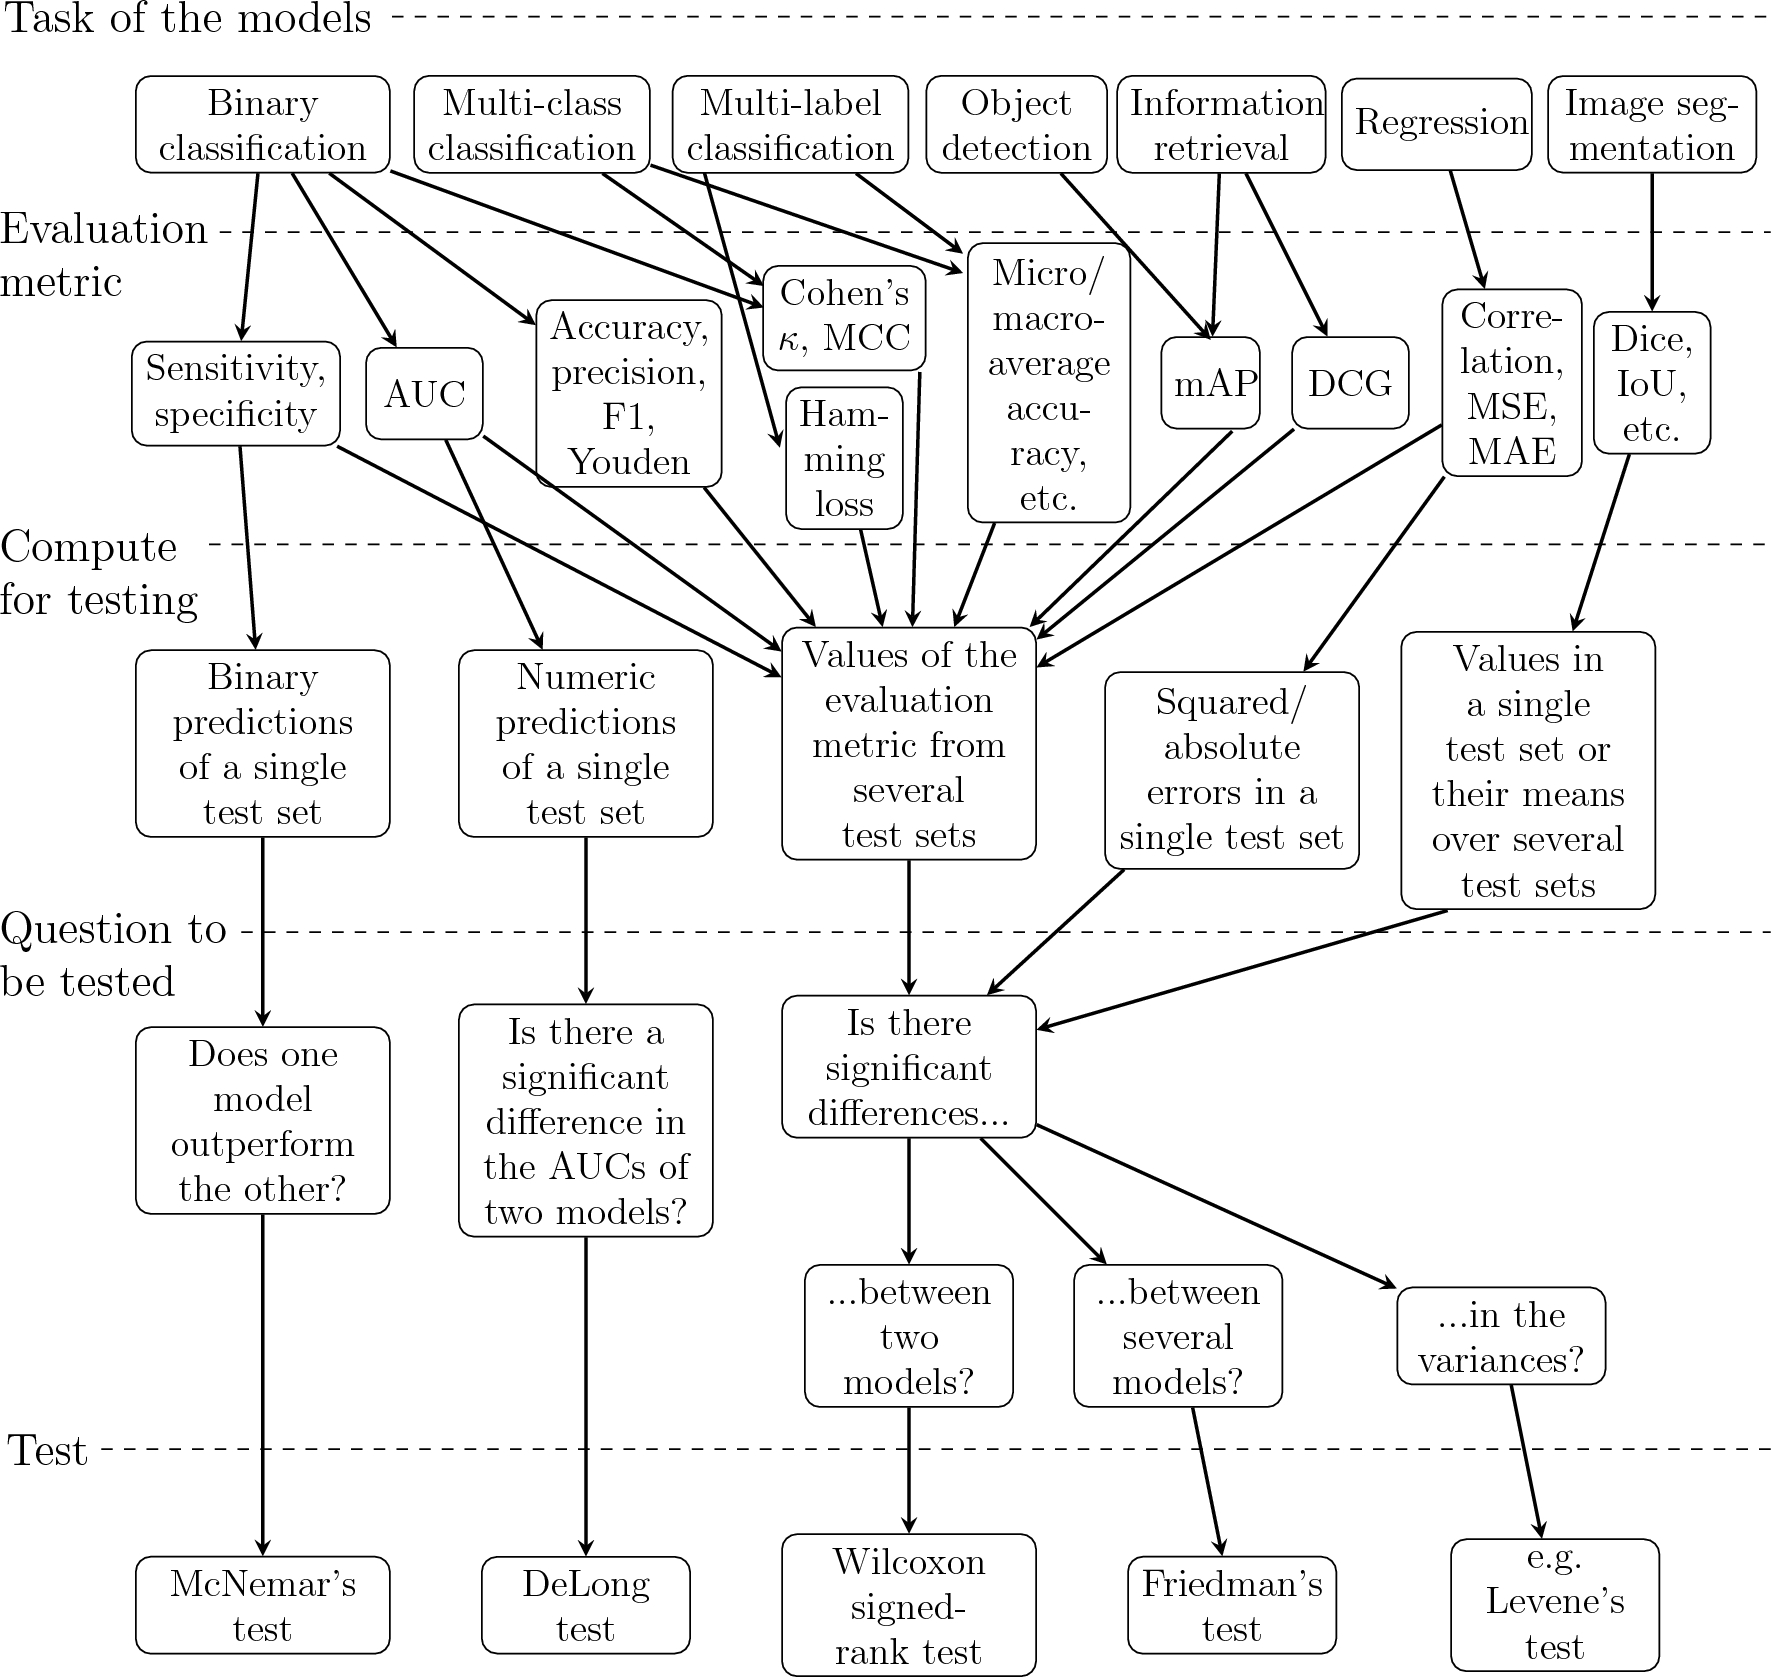
\includegraphics[totalheight=8cm]{images/41598_2024_56706_Fig3_HTML.png}
  \caption{Statistcal Workflow Provided by Rainio, Tauho, and Klén\cite{statsBased}}
  \label{fig:statistical test workflow}
\end{figure}
 
The Sentence\_Labeling sheet of the PsyTAR dataset used in this study is provided by Zoolnoori et al\cite{psyTAR1} and Zoolnori et al\cite{psyTar2}. This sheet contains three sections of interest. The first is sentences from online patient reviews of certain drugs. The second is annotations of certain labels, described below in table \ref{tab:6Labels}. The third is drug labels, which indicates which drug each sentence is reviewing.

Two classification tasks were performed using a baseline logistic regression model and a transformer model. The multi label class predicts six binary annotations, while the multi-class predicts four different drugs. For each model, different features will be used as inputs. The resulting predictions will be used for statistical tests in order to determine their statistical signifance. Specific details are described in the methods section.


%==============================
\section{Methods}\label{methods}
%==============================
% ASK ON WHETHER I NEED TO DESCRIBE IN DETAIL THE STATISTCAL TESTS USED
\subsection{Preprocessing}
Two main preprocessing steps were done. Firstly, as the drug labels in the data were concatenated with review ID, the review ID was stripped and only the drug label was added to a new column. Secondly, the review text was preprocessed through tokenization, as well as stopword and punctuation removal. The dataset consists of 6009 records. The data was split into train, validation, and test sets using a 45:45:10 ratio.
\subsection{Multi-Label Classification}
Multi-label classification involves predicting six labels, as shown in table \ref{tab:6Labels}. Each label is a binary task (1 for present and 0 for absent), which has been manually annotated. This task aims to predict annotations for a given review text.

\begin{table}[H]
  \centering
  \begin{tabular}{|p{4cm}|p{3cm}|}
    \hline
    \textbf{Predicted Class} & \textbf{Description} \\
    \hline
    Adverse Drug Reactions (ADR) & - \\
    \hline
    Withdrawal Symptom (WD) & - \\
    \hline
    Effective (EF) & - \\
    \hline
    Ineffective (INF) & - \\
    \hline
    Sign/Symptom/Illness (SSI) & Text contains explicit SSI as a result of the drug \\
    \hline
    Drug Indication (DI) & Text contains SSI that is currently being addressed by the drug \\
    \hline
  \end{tabular}
  \caption{The six labels predicted by multi-label classifiers}
  \label{tab:6Labels}
\end{table}

\subsubsection{Selected Features}

Two features were used for multi-label classification. The first is the preprocessed sentences without any additional features. From here on, references to this task-feature pair will be referred as Task\_1\_Feature\_1. The second contains the drug name added to the start of the review text. This will be referred to as Task\_1\_Feature\_2.

\subsubsection{Logistic Regression}
The logistic regression model performed Term Frequency Inverse Document Frequency (TF-IDF) vectorization on the input text. A multi-output classifier was built upon a logistic regression model, which was then tuned using hyperparameter tuning.

\subsubsection{Transformer}
The transformer model uses a pre-trained BERT model, which was trained on a downstream task in order to create a multi-label transformer classifier. Table \ref{tab:task1Parameters} shows the configurations used in the transformer.

\begin{table}[H]
  \centering
  \begin{tabular}{|p{4cm}|p{3cm}|}
    \hline
    \textbf{Parameter} & \textbf{Value} \\
    \hline
    hidden\_size & 768 \\
    \hline
    num\_hidden\_layers & 24 \\
    \hline
    num\_attention\_heads & 12 \\
    \hline
    intermediate\_size & 3072 \\
    \hline
    num\_labels & 6 \\
    \hline
    optimizer & AdamW \\
    \hline
  \end{tabular}
  \caption{BERT Configuration for Multi-Label Classification}
  \label{tab:task1Parameters}
\end{table}

\subsubsection{Statistical Tests}
Multi-class classification will be tested using macro and micro averaged precision, recall, and F1-scores. Accuracy will also be reported.

\textbf{Accuracy, Precision, Recall, and F1-Scores:}
\begin{equation}
  Accuracy = \frac{TP+TN}{TP+TN+FP+FN}
\end{equation}

\begin{equation}
  Precision = \frac{TP}{TP+FP}
\end{equation}

\begin{equation}
  Recall = \frac{TP}{TP+FN}
\end{equation}

\begin{equation}
  F1 = \frac{2*Precision*Recall}{Precision+Recall} = \frac{2*TP}{2*TP+FP+FN}
\end{equation}

In addition, follwing figure \ref{fig:statistical test workflow}, the Hamming Loss (HL) of the predictions are also calculated. HL measures the fraction of labels that are incorrectly predicted, on average, across all samples and is used to evaluate multi-label classification tasks\cite{hammingloss}.

\[
\text{HL} = \frac{1}{N \times L} \sum_{l=1}^L \sum_{i=1}^N (Y_{i,l} \neq X_{i,l})
\]

\begin{flalign*}
\text{where:} \\
N & : \text{Number of samples} \\
L & : \text{Number of labels} \\
Y_{i,l} & : \text{True label for } i\text{th sample and } \\ 
& l\text{th label} \\
hat{y}_{ij} & : \text{Predicted label for } i\text{th sample and }\\
& l\text{th label} \\
(Y_{i,l} \neq hat{y}_{ij}) & : \text {1} \text{ if } y_{ij} \neq \hat{y}_{ij} \text{ and } 0 \text{ otherwise}
\end{flalign*}

\subsection{Multi-Class Classification}
Multiclass classification aims to take in text and predict the drug that is being reviewed. There are four classes of drugs to predict. Lexapro, cymbalta, effexorxr, and zoloft.

\subsubsection{Selected Features}

Three features were selected for multi-class classification. The first is the preprocessed sentence without any additional features, referred to as Task\_2\_Feature\_1. 

The second is the preprocessed text along with its annotations. For the logistic regression model, the binary annotations are simply added onto the end of the sentences as 1s and 0s. 

On the other hand, the transformer's input has the review text concatenated with the predicted class names. If the class is labelled 1, a [POS] token was placed in front of it. If the class is labelled 0, a [NEG] token was placed instead. These tokens identify positive(1) and negative(0) labels respectively. This feature will be referred to as Task\_2\_Feature\_2. References to this task-feature pair will be described with the model (e.g., Task\_2\_Feature\_2(Transformer)) when the specifc model feature is of importance. Otherwise, Task\_2\_Feature\_2 will refer to this task-feature pair generally.

The third feature is to only use the annotation inputs. This will be referred to as Task\_2\_Feature\_3. Similar to feature 2, the logistic regression takes in binary labels while the transformer takes in predicted class names with the described tokens above. Similar references to specific or general model will be made for this task-feature pair.

\subsubsection{Logistic Regression}

TF-IDF was also used on the input text. However, in contrast to using a multi-label classifier built on top of a logistic regression model, multi-class classification uses logistic regression directly.

\subsubsection{Transformer}
The transformer model is identical to the multi-label transformer, except it was trained on a multi-class downstream task. The number of hidden layers was also decreased due to long training times (about 1 hour for 1 epoch using 24 layers on a NVIDIA GeForce RTX 3060 Ti). The transformer specifications are shown in table \ref{tab:task2Parameters}.

\begin{table}[H]
  \centering
  \begin{tabular}{|p{4cm}|p{3cm}|}
    \hline
    \textbf{Parameter} & \textbf{Value} \\
    \hline
    hidden\_size & 768 \\
    \hline
    num\_hidden\_layers & 8 \\
    \hline
    num\_attention\_heads & 12 \\
    \hline
    intermediate\_size & 3072 \\
    \hline
    num\_labels & 1 \\
    \hline
    optimizer & AdamW \\
    \hline
  \end{tabular}
  \caption{BERT Configuration for Multi-Class Classification}
  \label{tab:task2Parameters}
\end{table}
\subsubsection{Statistical Tests}
Multi-class classification will be tested using macro and micro averaged precision, recall, and F1-scores as described previously. Accuracy will also be reported.

Additionally, following figure \ref{fig:statistical test workflow}, Cohen's Kappa (Cohen's K) and Matthews Correlation Coefficient (MCC) will be used. 

Cohen's K is calculated using the following formula: 

\textbf{Cohen's K:}

\begin{equation}
  \kappa = \frac{p_o - p_e}{1 - p_e}
  \end{equation}
  
  where:
  \begin{align*}
  p_o & = \text{relative observed agreement among raters} \\
  p_e & = \text{hypothetical probability of chance agreement}
  \end{align*}
  
  ($p_o$) is calculated as:
  
  \begin{equation}
  p_o = \frac{a + d}{a + b + c + d}
  \end{equation}
  
  ($p_e$) is calculated as:
  
  \begin{align}
    p_e &= \left(\frac{(a + b)}{a + b + c + d} \cdot \frac{(a + c)}{a + b + c + d}\right) \notag \\
    &\quad + \left(\frac{(c + d)}{a + b + c + d} \cdot \frac{(b + d)}{a + b + c + d}\right)
    \end{align}

  where:
  \begin{itemize}
      \item $a$ = Number of times both annotators agreed the sample was positive
      \item $d$ = Number of times both annotators agreed the sample was negative
      \item $b$ = Number of times Annotator A said positive but Annotator B said negative
      \item $c$ = Number of times Annotator A said negative but Annotator B said positive
  \end{itemize}

Cohen's K returns a value between 1 and -1, where 1 means a perfect agreement, 0 means no agreement above chance, and -1 indicating agreement less than chance. Cutoff points for Cohen's K is given in table \ref{tab:kappaInterpretation}, which is based on McHugh's research\cite{cohen}.

\begin{table}[H]
  \centering
  \begin{tabular}{|p{4cm}|p{3cm}|}
    \hline
    \textbf{Absolute Cohen's Kappa Range} & \textbf{Interpretation} \\
    \hline
    $|\kappa| \leq 0$ & No agreement \\
    \hline
    $0.01 \leq |\kappa| \leq 0.20$ & None to slight agreement \\
    \hline
    $0.21 \leq |\kappa| \leq 0.40$ & Fair agreement \\
    \hline
    $0.41 \leq |\kappa| \leq 0.60$ & Moderate agreement \\
    \hline
    $0.61 \leq |\kappa| \leq 0.80$ & Substantial agreement \\
    \hline
    $0.81 \leq |\kappa| \leq 1.00$ & Almost perfect agreement \\
    \hline
  \end{tabular}
  \caption{Cohen's Kappa Cutoff Points}
  \label{tab:kappaInterpretation}
\end{table}


MCC is used to measure the quality of binary classifications\cite{mcc}. The formula for MCC is given:

\textbf{MCC:}
\begin{equation}
  \resizebox{0.9\hsize}{!}{$
  \text{MCC} = \frac{TP \cdot TN - FP \cdot FN}{\sqrt{(TP + FP)(TP + FN)(TN + FP)(TN + FN)}}
  $}
  \end{equation}

Similar to Cohen's K, MCC returns a value betwen 1 and -1, where 1 means perfect predictions, 0 means a prediction that is no better than random, and -1 means total disagreement between predictions and observations. While the cutoff points of MCC are generally created using a receiver operating characteristic (ROC) curve, this report will follow a basic cutoff point described in table \ref{tab:mccInterpretation}.

\begin{table}[H]
  \centering
  \begin{tabular}{|p{4cm}|p{3cm}|}
    \hline
    \textbf{Absolute MCC Values} & \textbf{Interpretation} \\
    \hline
    $0 \leq |\text{MCC}| \leq 0.1$ & Random Performance \\
    \hline
    $0.1 < |\text{MCC}| < 0.3$ & Weak Correlation \\
    \hline
    $0.3 \leq |\text{MCC}| < 0.5$ & Moderate Correlation \\
    \hline
    $|\text{MCC}| \geq 0.7$ & Strong Correlation \\
    \hline
  \end{tabular}
  \caption{MCC Cutoff Points}
  \label{tab:mccInterpretation}
\end{table}

\subsection{Friedman's Test of Significance}
In order to investigate whether the predictions are significantly different from each other, Friedman's test will be performed on both tasks. Friedman's test is a hypothesis testing method, where the null hypothesis is that there is no significant difference between two samples of predictions. Meanwhile, the alternative hypothesis is that a significant difference does exist. This test returns a probability(p)-value, which indicates how likely is it to get result predictions if the compared samples have no significant differences. A cutoff point ($\alpha$ value) of 5\% will be used, meaning that if the p-value is <5\%, the null hypothesis will be rejected.

\textbf{Friedman's Test:}

\begin{equation}
  T = \frac{12 \sum S_{ij}^2}{jk(j+1)} - 3k(j+1)
\end{equation}

where:
\begin{align*}
T & = \text{test statistic} \\
\sum S_{ij}^2 & = \text{sum of the squared sums of ranks for each prediction set} \\
j & = \text{number of prediction sets} \\
k & = \text{number of instances}
\end{align*}


%==============================
\section{Results}\label{results}
%==============================

%==============================
\section{Discussion and Conclusion}\label{discussion and conclusion}
%==============================
% future work could include additional statistical tests on features (e.g., chi squared tests of feature indpendence) Efficient and inefficient obviously have some feature dependence, but these are labels. nevertheless, these could be investigated

%a challenge is that NLP tasks generally uses one singular text as the input (e.g.,just the review text). However, we still show how investigating feature engineering on the text could provide deeper insights on how the model performs and increases interpretability.
%==============================
\bibliographystyle{vancouver}
\bibliography{literature}
%==============================

\section{Appendix}

\end{document}